% !TEX encoding = UTF-8
%Koma article
\documentclass[fontsize=12pt,paper=letter,twoside]{scrartcl}
\usepackage{float}
\usepackage{listings}

%Standard Pre-amble
\usepackage[top=4cm,bottom=4cm,left=3cm,right=3cm,asymmetric]{geometry}
%\geometry{landscape}                % Activate for for rotated page geometry
%\usepackage[parfill]{parskip}    % Begin paragraphs with an empty line rather than an indent
\usepackage[table,xcdraw]{xcolor}
\usepackage{graphicx}

\usepackage{amsmath}
\usepackage{amssymb}
\usepackage{epstopdf}
\DeclareGraphicsRule{.tif}{png}{.png}{`convert #1 `dirname #1`/`basename #1 .tif`.png}
% Listings needs package courier
\usepackage{listings} % Needs 
\usepackage{courier}

\usepackage[framemethod=TikZ]{mdframed}
\usepackage{url}

\usepackage{sty/bsymb} %% Event-B symbols
\usepackage{sty/eventB} %% REQ and ENV
\usepackage{sty/calculation}

%Maths
\usepackage{amssymb,amsmath}
\def\Fl{\mathbb{F}}
\def\Rl{\mathbb{R}}
\def\Nl{\mathbb{N}}
\def\Bl{\mathbb{B}}
\def\St{\mathbb{S}}
\newcommand{\ovr}{\upharpoonright}
\newcommand{\var}[1]{\textit{#1}}
%Useful definitions
\newcommand{\mv}[1]{\textit{m\_#1}}
\newcommand{\cv}[1]{\textit{c\_#1}}
\newcommand{\degree}[1]{^{\circ}\mathrm{#1}}
%\newcommand{\comment}[1]{{\footnotesize \quad\texttt{--}\textrm{#1}}}
\newcommand{\im}[1]{i\texttt{-\!#1}}

\usepackage[headsepline]{scrpage2}
\pagestyle{scrheadings}
\ihead[]{\small EECS4312 Report1}
\ohead[]{\small \thepage}
\cfoot[]{}
\ofoot[]{}


%%%%PVS environment%%%%%%%%%%%%%%%%%%%
\lstnewenvironment{pvs}[1][]
    {\lstset{#1,captionpos=b,language=pvs,
    mathescape=true,
    basicstyle=\small\ttfamily,
    numbers=none,
    frame=single,
    % numberstyle=\tiny\color{gray},
    % backgroundcolor=\color{lightgray},
    firstnumber=auto
    }}
    {}
 %%%%%%%%%%%%%%%%%%%%%%%%%%%%%%%%
 
%%%%Verbatim environment%%%%%%%%%%%%%%%%%%%
\lstnewenvironment{code}[1][]
    {\lstset{#1,captionpos=b,
    mathescape=true,
    basicstyle=\small\ttfamily,
    numbers=none,
    frame=single,
    % numberstyle=\tiny\color{gray},
    % backgroundcolor=\color{lightgray},
    firstnumber=auto
    }}
    {}

% \newenvironment{boxed}[1]
%    {\begin{center}
%    #1\\[1ex]
%    \begin{tabular}{|p{0.9\textwidth}|}
%    \hline\\
%    }
%    { 
%    \\\\\hline
%    \end{tabular} 
%    \end{center}
%    }
 %%%%%%%%%%%%%%%%%%%%%%%%%%%%%%%%
 
 %Text in a box
\newenvironment{textbox}
    {\begin{center}
    \begin{tabular}{|p{0.9\textwidth}|}
    \hline\\
    }
    { 
    \\\\\hline
    \end{tabular} 
    \end{center}
    }

\usepackage{hyperref}

%Highlight \hl{}
\usepackage{soul}

\usepackage{enumitem}
\newlist{mylist}{itemize}{1}
\setlist[mylist]{label=\textbullet,leftmargin=1cm,nosep}

\usepackage{multirow}

% Reduce space between figure and caption
%\usepackage{caption}
%\captionsetup[table]{font=small,skip=0pt}     %% Adjust here
%or equivalently 
\usepackage[font=small,skip=4pt]{caption}
%Useful definitions
%\newcommand{\mv}[1]{\textit{m\_#1}}
%\newcommand{\cv}[1]{\textit{c\_#1}}
%\newcommand{\degree}[1]{^{\circ}\mathrm{#1}}
%\newcommand{\comment}[1]{{\footnotesize \quad\texttt{--}\textrm{#1}}}

% Set the header
\ihead[]{\small EECS4090 Project}


%%%%%%%%%%%%Enter your names here%%%%%%%%
\author{\textbf{Edward Vaisman}
\and \textbf{Sadman Sakib Hasan}
}
%%%%%%%%%%%%%%%%%%%%%%%%%%%%%%%%

\date{\today} % Display a given date or no date

\begin{document}
\title{Grad Apps 2.0 \\ Professor User Manual}
\maketitle

\newpage

%%%%%%%%%%%%%%%%%%%%%%%%%%%%%%%
\tableofcontents

\newpage


%%%%Rest of your document goes here%%%%%%%%%%%%%%%%%%%

\clearpage
\section{Logging In}

To access the gradapps portal you'll first need to be authenticated into the system. To begin simply click on the ``Sign In" button on the welcome page.

\begin{figure}[!htb]
\begin{center}

\includegraphics[width=.99\textwidth]{images/welcome.png}
\end{center}
\caption{Welcome Page}
\label{fig:welcome}
\end{figure}

\bigskip

You will then be redirected to the login page. Input your username, password and click on the ``Login" button. If you are successfully authenticated you will be redirected to the role selection page.

\begin{figure}[!htb]
\begin{center}
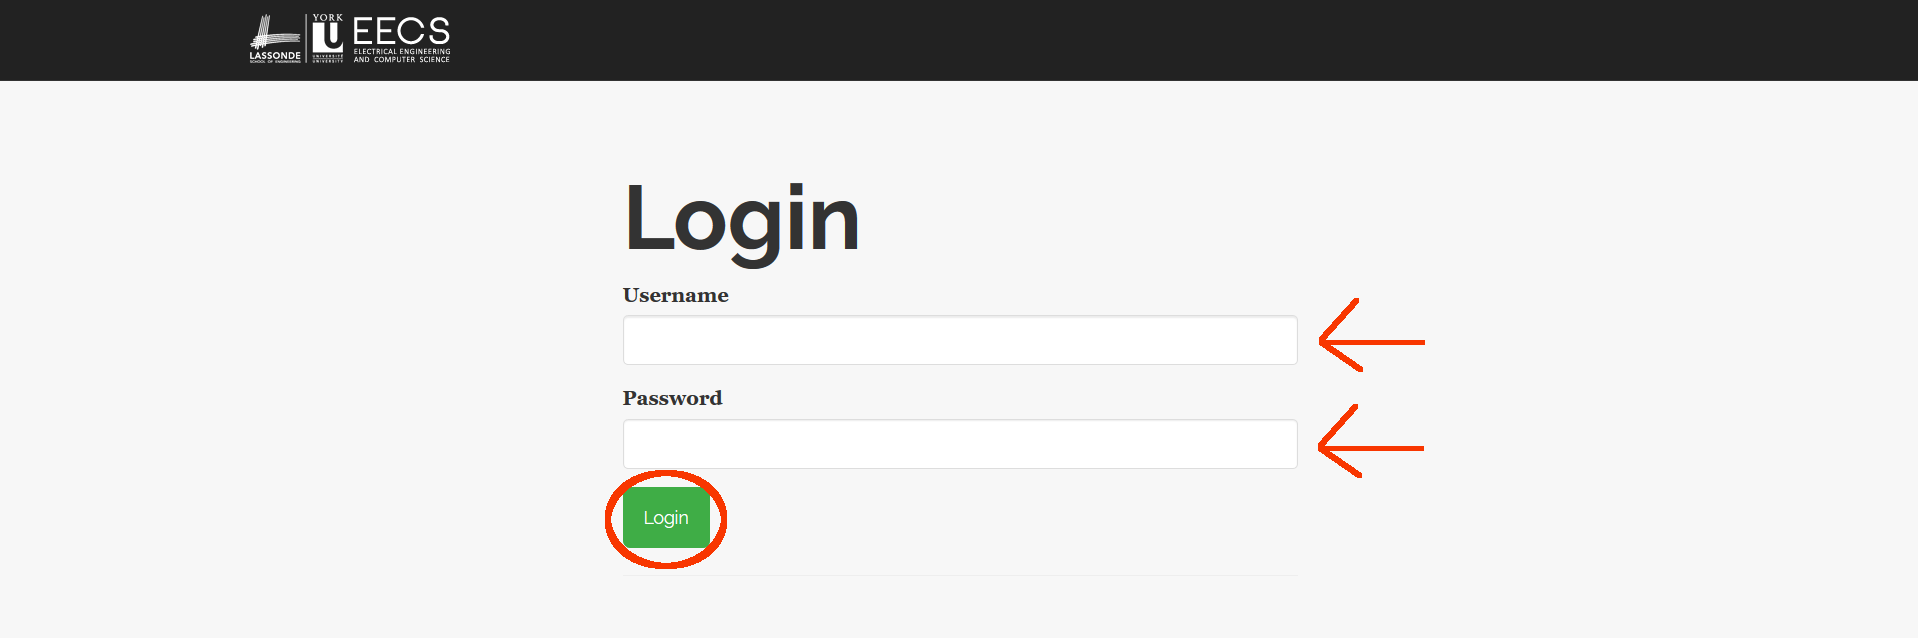
\includegraphics[width=.99\textwidth]{images/login.png}
\end{center}
\caption{Login Page}
\label{fig:login}
\end{figure}
\noindent \textbf{Note:} If the credentials you have provided are invalid you will be greeted with an error message.

\clearpage

\section{Selecting a Role}
The subsections below describe the methods for selecting the a role.

\subsection{Role Selection Page}
From the role selection page click on the ``Continue as Professor" button to be redirected to the professor portal.

\begin{figure}[!htb]
\begin{center}
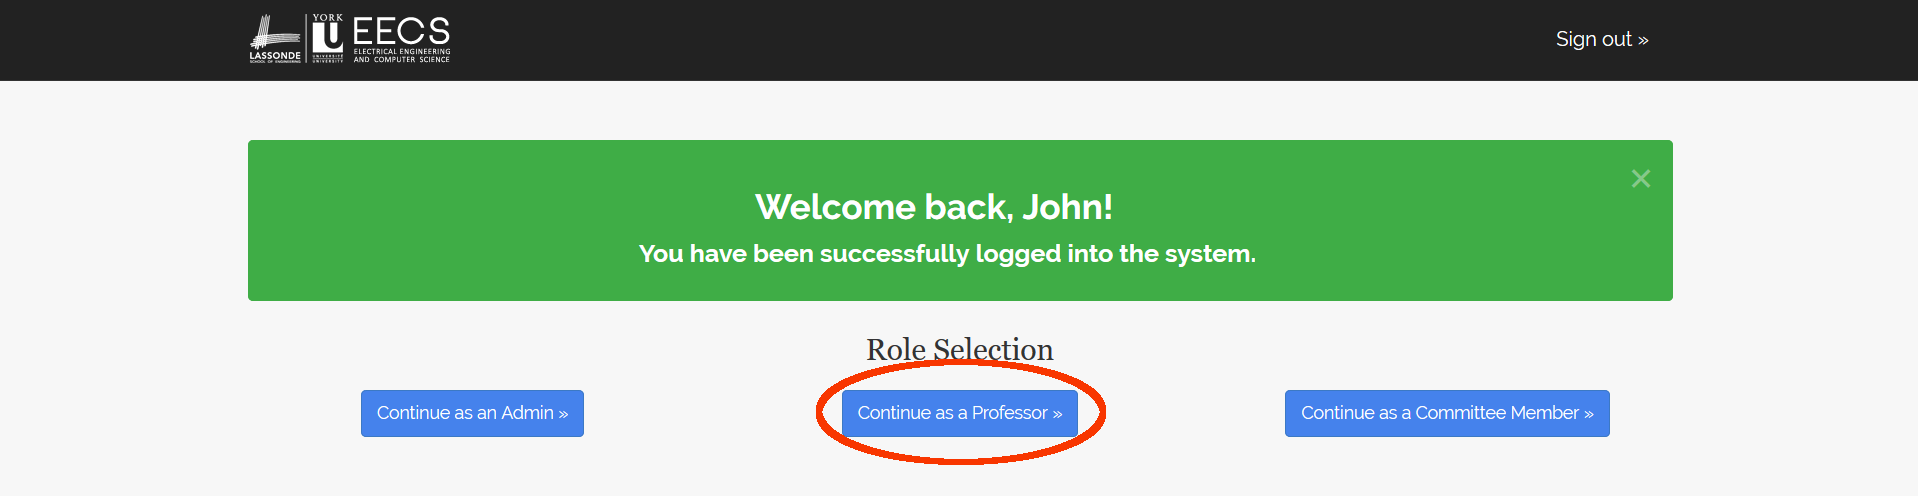
\includegraphics[width=.99\textwidth]{images/role-selection.png}
\end{center}
\caption{Role Selection Page}
\label{fig:role_selection1}
\end{figure}

\noindent \textbf{Note:} To access the administrator/committee/professor portal you must be granted access from an administrator.

\subsection{Navigation Bar}
If you have selected another role and wish to switch roles you will be presented with an option on the navigation bar. Click on the dropdown menu that displays your current role and click on your desired role.
\begin{figure}[!htb]
\begin{center}

\includegraphics[width=.99\textwidth]{images/role-selection2.png}
\end{center}
\caption{Switch Roles}
\label{fig:role_selection2}
\end{figure}

\noindent \textbf{Note:} To access the administrator/committee/professor portal you must be granted access from an administrator.

\clearpage

Once you have selected the professor role you will should see a page similar to the one below

\begin{figure}[!htb]
\begin{center}
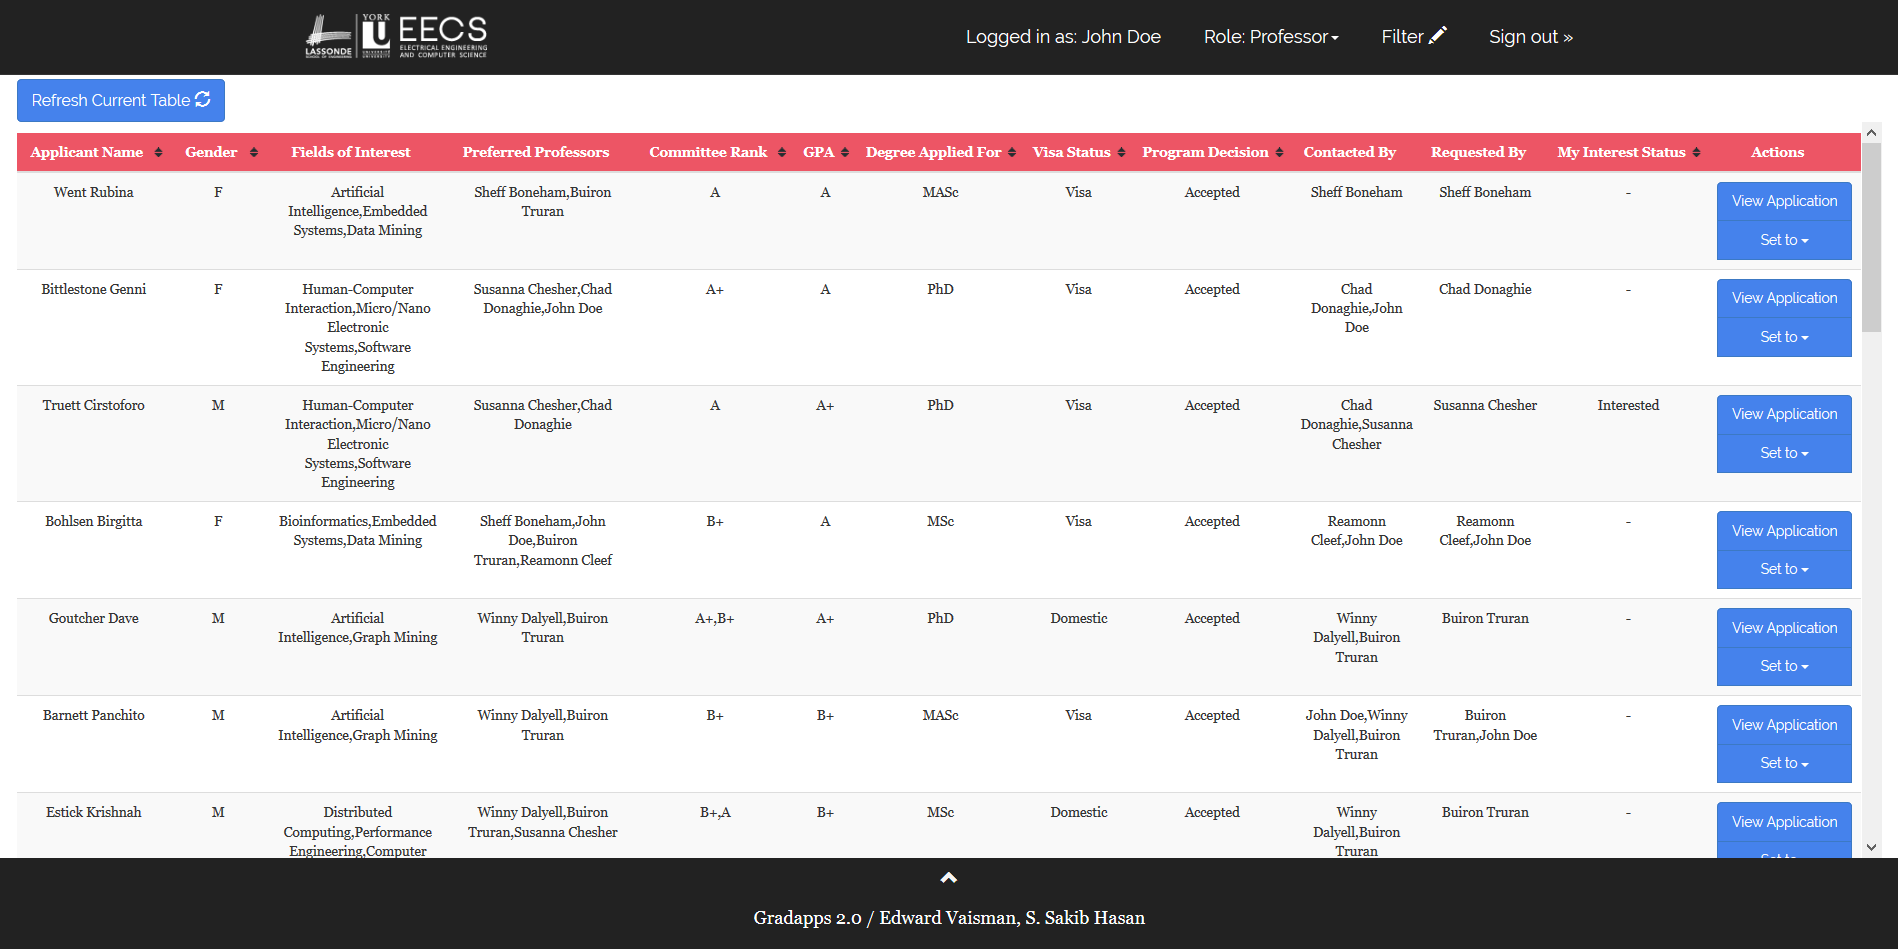
\includegraphics[width=.99\textwidth]{images/professor.png}
\end{center}
\caption{Professor Portal}
\label{fig:professor}
\end{figure}

\clearpage
\section{Professor Portal}
After logging in and selecting the professor role you will the have access to the professor portal. In this portal you will be presented with a table containing all the students who have applied to be a graduate student. Here you can perform the following:
\begin{itemize}
\item Filter the table to only display applications based on a criteria of your choosing
\item Sort the table on certain columns
\item View the applicants application and their respective committee review
\item Set application attributes such as notifying others if you have contacted/requested an applicant or indicate to yourself if you find an applicant interesting or not.
\end{itemize} 
\subsection{Filtering the Table}
This section describes how you would use/build/save/load a filter on the table.


\begin{figure}[!htb]
\subsubsection{Opening the Modal}
To begin with filtering you must open the modal. To do so click on the ``Filter" button on the navigation bar.
\begin{center}
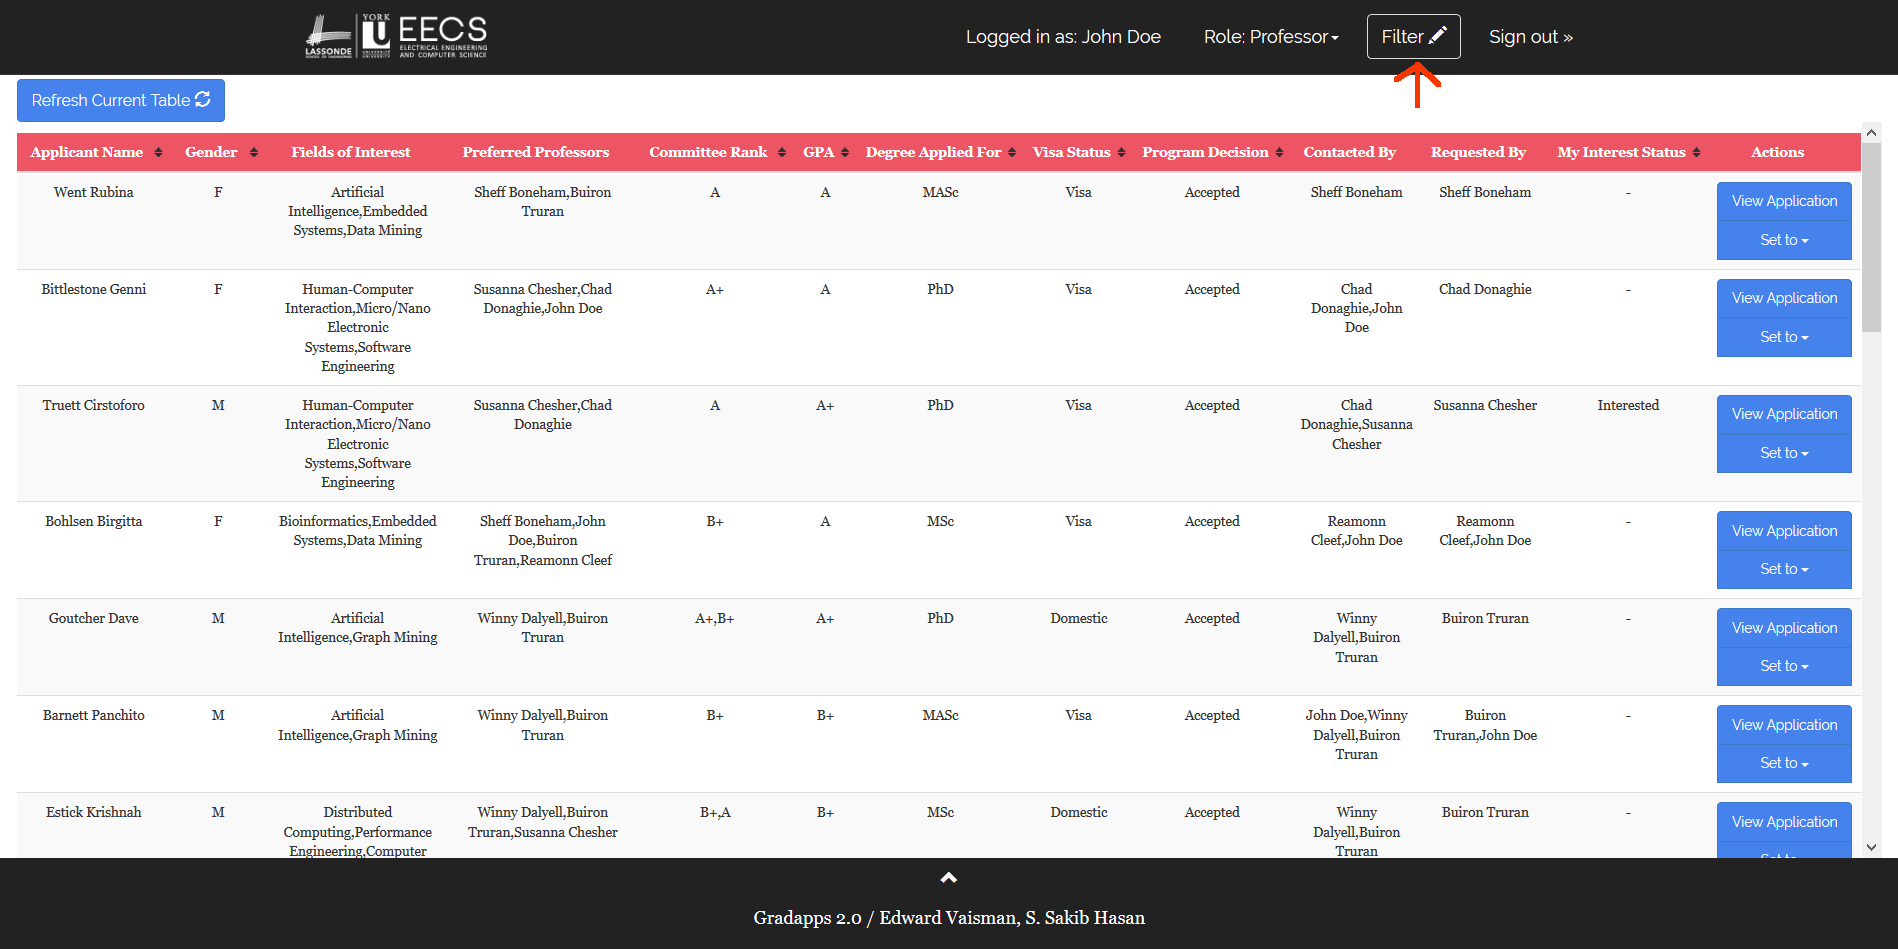
\includegraphics[width=.99\textwidth]{images/open_modal.png}
\end{center}
\caption{Opening the  Modal}
\label{fig:open_modal}
\end{figure}
\clearpage

\begin{figure}[!htb]
\begin{center}
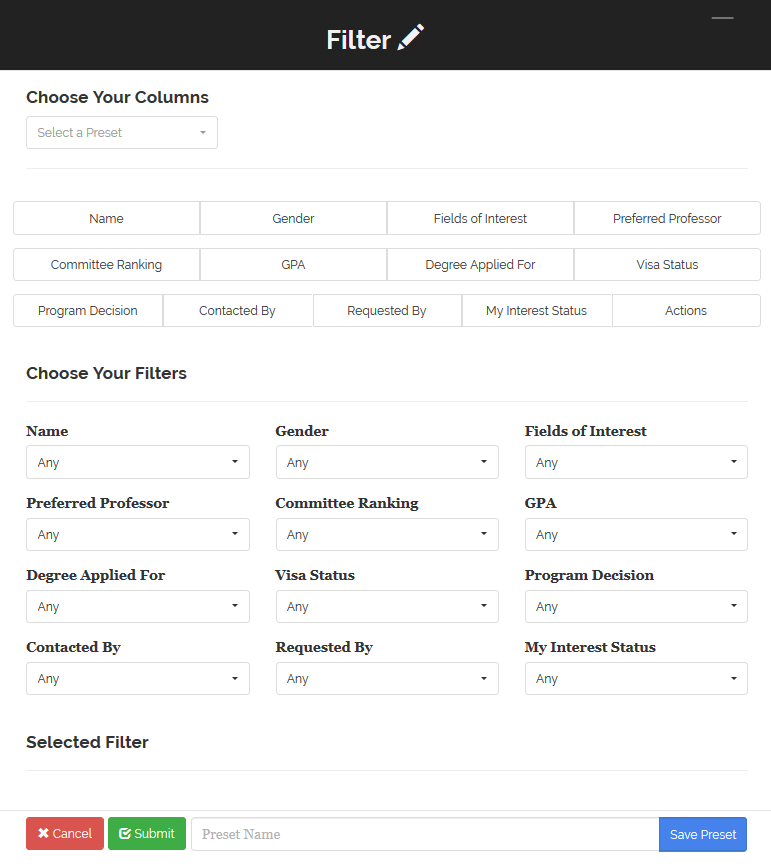
\includegraphics[width=.99\textwidth]{images/filter_view.png}
\end{center}
\caption{Filter View}
\label{fig:filter_view}
\end{figure}

\clearpage
\begin{figure}[!htb]
\subsubsection{Choose Your Columns}
Once the modal is opened you can then choose the columns you wish to be displayed on the table. To do so, click on the button indicating which column you wish to see. Once clicked the button will display the order that column will appear in the table.\begin{center}
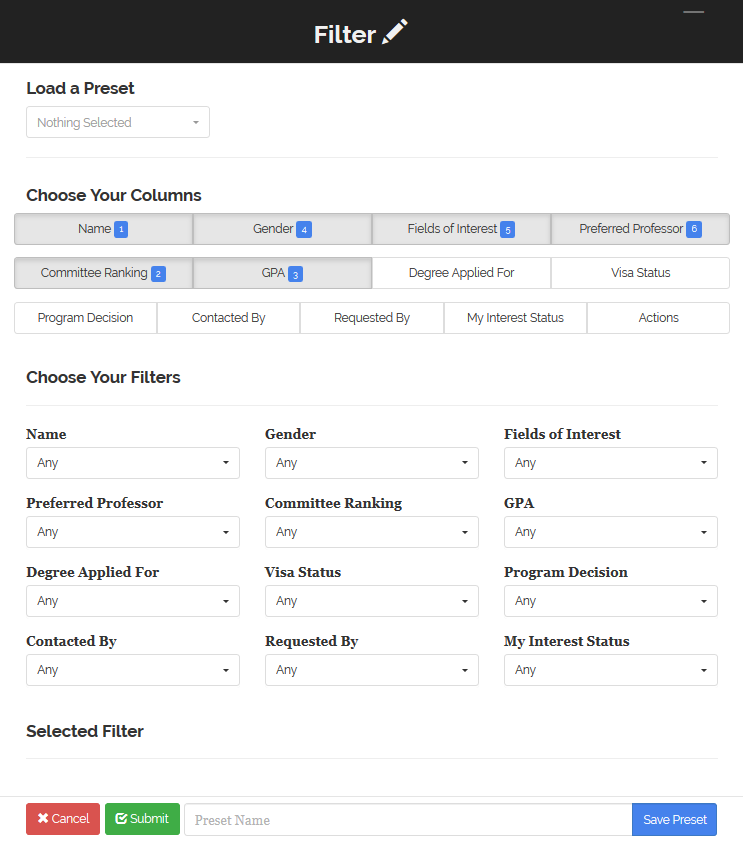
\includegraphics[width=.99\textwidth]{images/choose_columns.png}
\end{center}
\caption{Choose Your Columns}
\label{fig:choose_columns}
\textbf{Note:} Not selecting any column will use the same columns and order of the default table. If the \emph{Actions} column is not selected it will automatically be placed to the right most column. \emph{My Interest Status} is account specific and can only be seen by you.
\end{figure}

\clearpage

\begin{figure}[!htb]
\subsubsection{Choose Your Filters}
After selecting your columns, you can then choose the attributes you wish to filter your table by. Begin by clicking on the drop down of the attribute you which to filter and select an option from a list of generated options.
\begin{center}
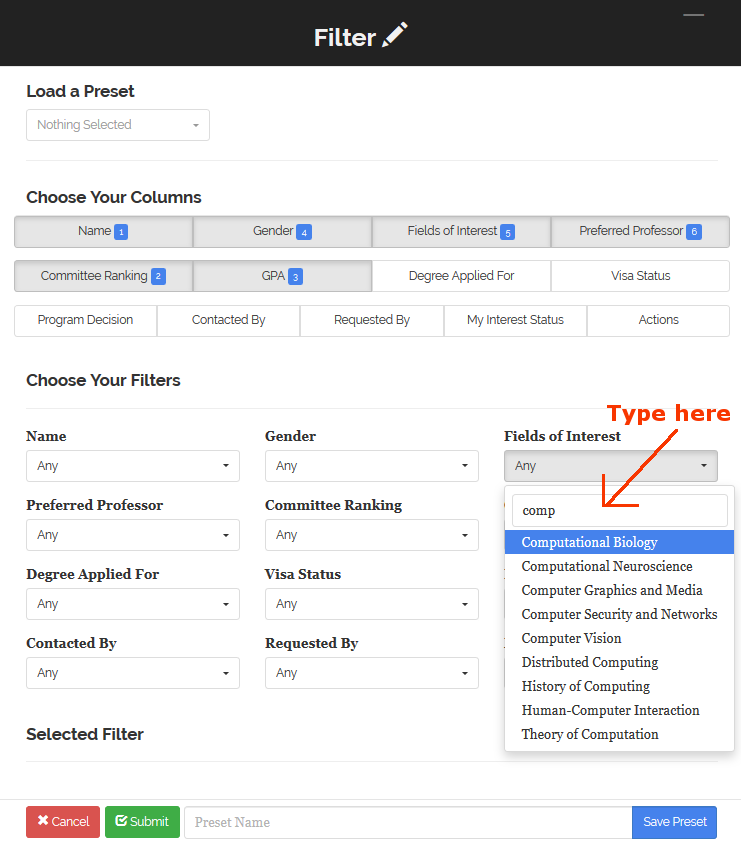
\includegraphics[width=.99\textwidth]{images/choose_filters.png}
\end{center}
\caption{Choose Your Filters}
\textbf{Note:} You can use the search bar to help search for what you are looking for. Begin by typing in the text box displayed. You can only select an option that appears in the dropdown.
\label{fig:choose_filters}
\end{figure}

\clearpage 
\begin{figure}[!htb]
\subsubsection{Submitting a Filter}
Once you have chosen your columns and filter attributes confirm your filter by reading the text under ``Selected Filter'' and click ``Submit". The text under the ``Selected Filter'' will change based on your filter attributes.
\begin{center}
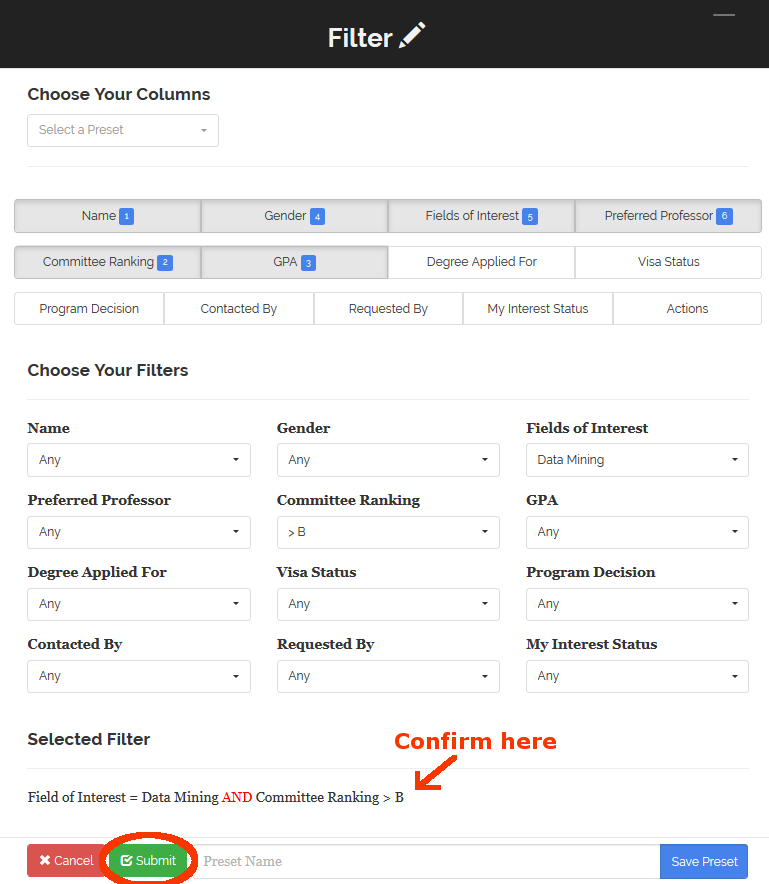
\includegraphics[width=.99\textwidth]{images/submit_filter.png}
\end{center}
\caption{Submit Filter}
\label{fig:submit_filter}
\end{figure}

\clearpage
After you submit a filter you will be provided with a new table to match your filter.
\begin{figure}[!htb]
\begin{center}
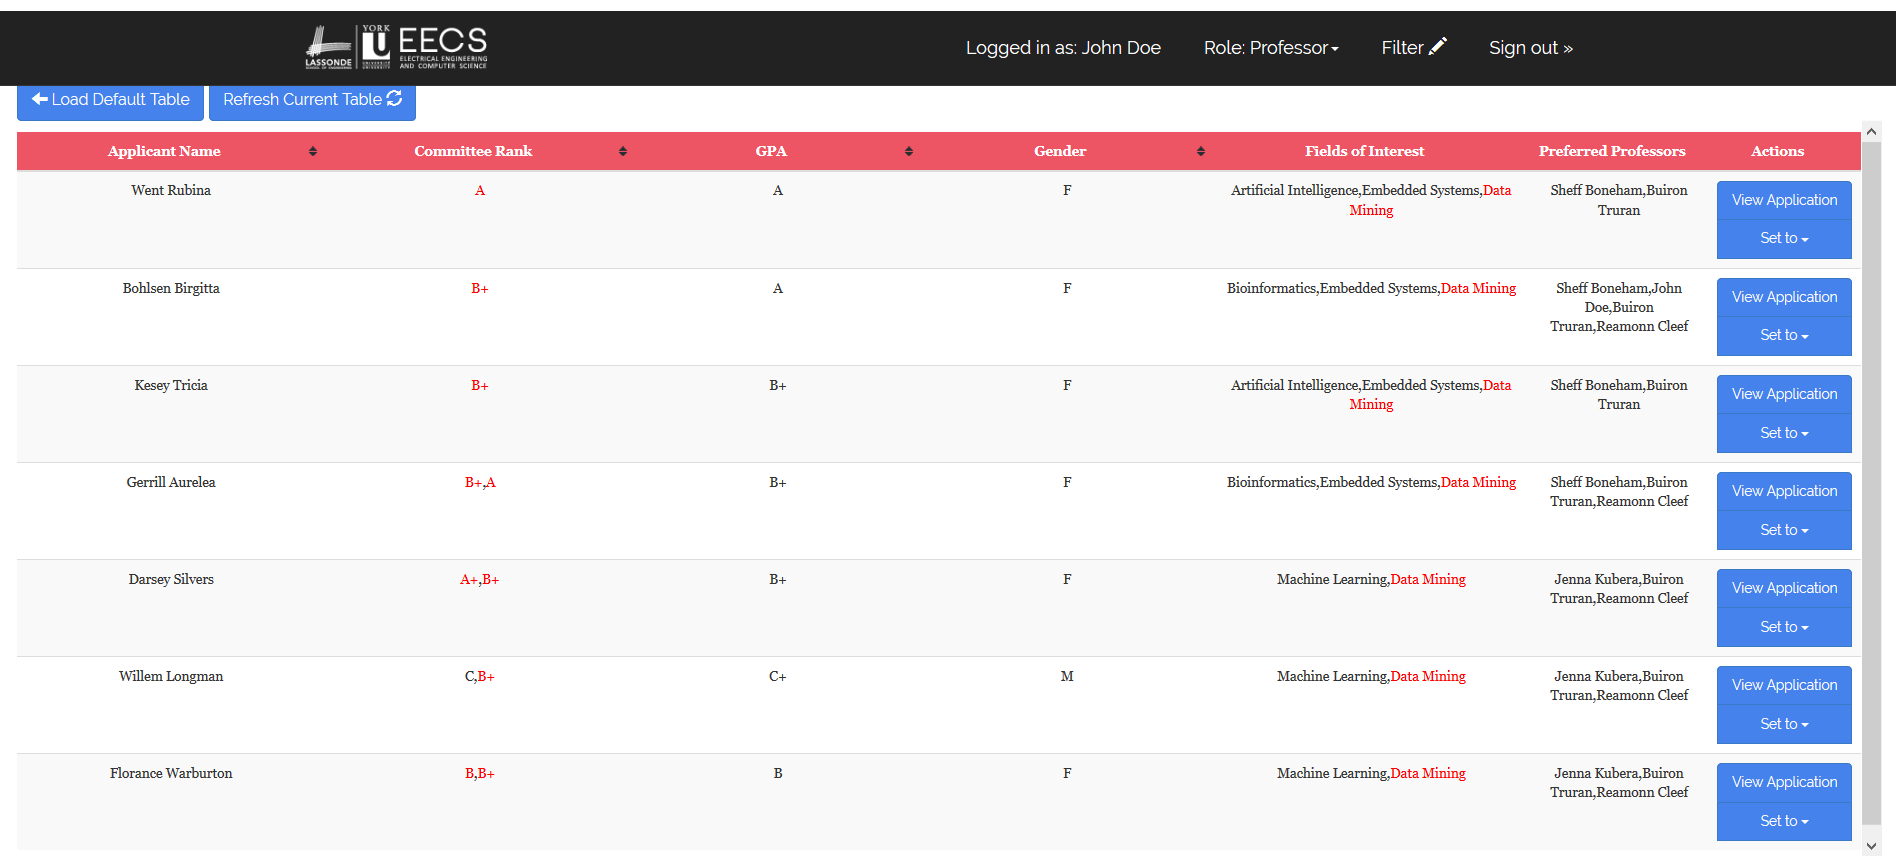
\includegraphics[width=.99\textwidth]{images/filtered_table.png}
\end{center}
\caption{Filtered Table}
\textbf{Pro-tip:} Attributes that satisfy your filter will be highlighted. Make sure to include the right column to see that highlights!
\label{fig:filtered_table}
\end{figure}

\clearpage 

\begin{figure}[!htb]
\subsubsection{Saving a Filter}
Once you have chosen your columns and filter attributes confirm your filter by reading the text under ``Selected Filter'' and give the preset a name by typing in the text box between the ``Submit'' and the ``Save Preset'' button. Once that is done click ``Save Preset''
\begin{center}
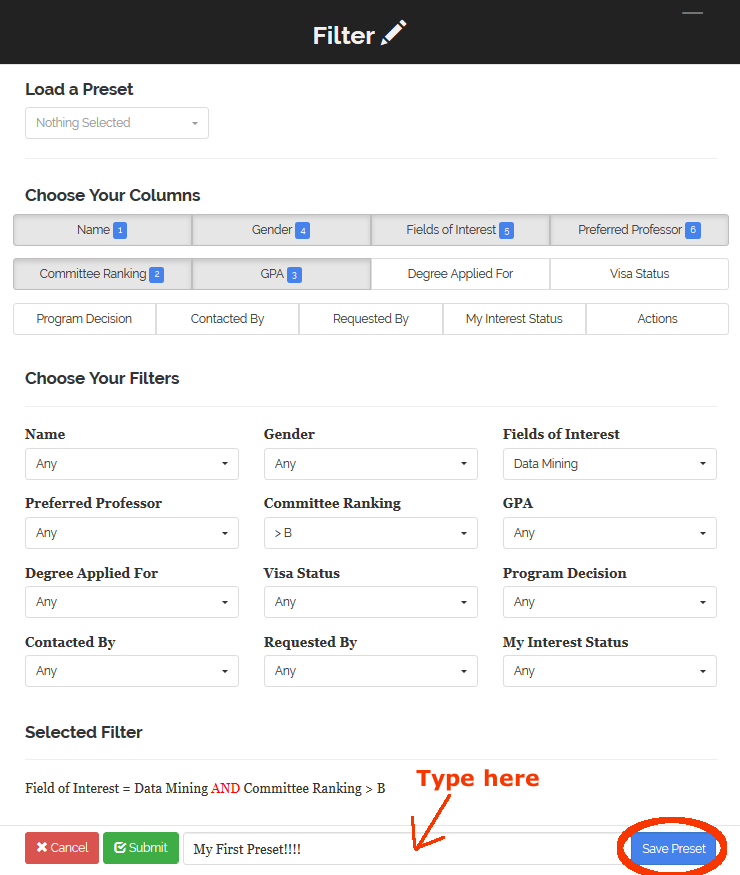
\includegraphics[width=.99\textwidth]{images/save_filter.png}
\end{center}
\caption{Save a Filter}
Once you have saved a filter you will be provided with a new table to match your filter and it will appear in the dropdown to be used for loading a filter.\\
\textbf{Pro-tip:} You can update a filter by typing in the same name as an existing filter.
\label{fig:save_filter}
\end{figure}

\clearpage
\begin{figure}[!htb]
\subsubsection{Loading a Filter}
To load a saved filter click the dropdown under ``Load a Preset'' and select the preset you wish to use. Once selected the modal will auto-populate
\begin{center}
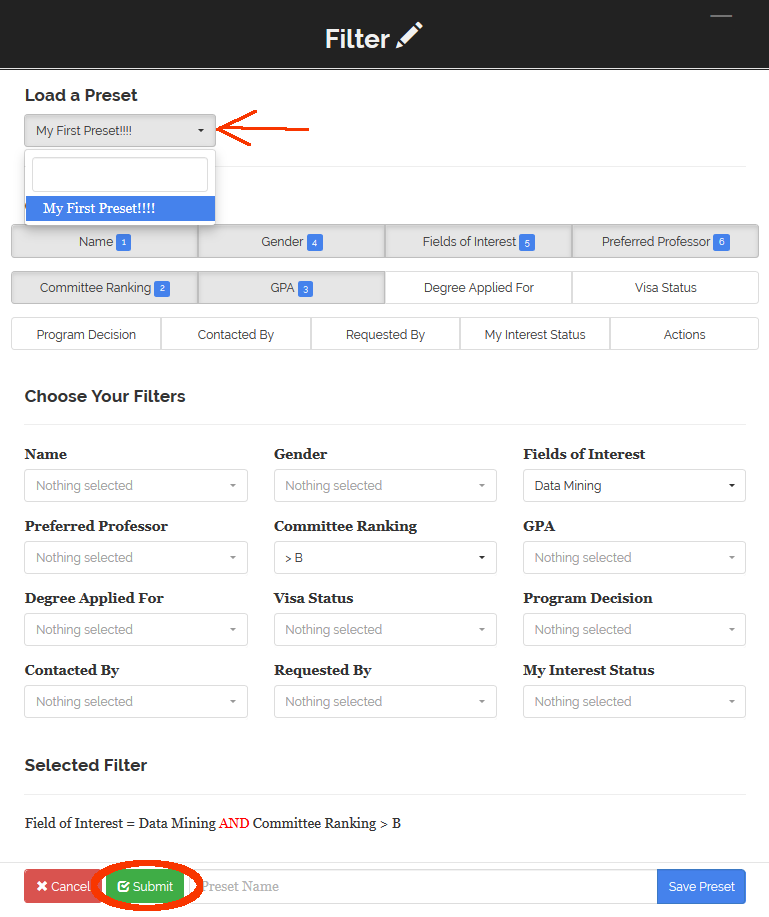
\includegraphics[width=.99\textwidth]{images/load_filter.png}
\end{center}
\caption{Loading a Filter}
\textbf{Pro-tip:} Create a preset called \emph{Default} with no columns or filters selected. You can then use this to load the default table or help clear any data you put in the modal.
\label{fig:save_filter}
\end{figure}

\clearpage

\subsection{Sorting the Table}
If you wish to sort the table displayed simply click on the columns that display arrows next to the name. The table can be sorted in Ascending/Descending order described below
\begin{itemize}
\item \textbf{Name:} Descending Order = Z to A, Ascending order = A to Z
\item \textbf{Gender:} Descending Order = Z to A, Ascending order = A to Z
\item \textbf{Committee Rank:} Descending Order = A+ to C, Ascending order = C to A+
\item \textbf{GPA:} Descending Order = A+ to C, Ascending order = C to A+
\item \textbf{Degree Applied For:} Descending Order = Z to A, Ascending order = A to Z
\item \textbf{Visa Status:} Descending Order = Z to A, Ascending order = A to Z
\item \textbf{Program Decision:} Descending Order = Z to A, Ascending order = A to Z
\item \textbf{Interest Status:} Descending Order = Z to A, Ascending order = A to Z
\end{itemize}
\textbf{Pro-tip:} To sort my multiple columns hold onto the shift key while clicking on the columns. For example to sort by Committee Rank then GPA hold onto shift and left click Committee Rank then GPA.
\subsection{Viewing an Application}
\subsection{Setting Application Attributes}
\subsubsection{Contacted By}
\subsubsection{Requested By}
\subsubsection{My Interest Status}


\end{document}
